\chapter{Predicting Murder Rates With Gradient Descent}

\section{Goal}

\begin{fullwidth}

The goal of this exercise is to extend the techniques you learned in the one-dimensional gradient descent task to a two-dimensional domain space, solving a {\em linear regression problem}.  This problem is also known as {\em curve fitting}.  As part of this lab, you will learn how to compute with vectors instead of scalars.

\section{Discussion}

\subsection{Problem statement}

Given training data $(x_i, y_i)$ for $i=1..n$ samples with dependent variable $y_i$, we would like to predict $y$ for some $x$'s not in our training set. $x_i$ is generally a vector of independent variables but we'll use a scalar. If we assume there is a linear relationship between $x$ and $y$, then we can draw a line through the data and predict future values with that line function. To do that, we need to compute the two parameters of our model: a slope and a $y$ intercept. (We will see the model below.)

For example, if we compare the number of murders per 100,000 people in Detroit to the average hourly wage, our eyeballs easily detect a correlation.  Here is data suitable to copy and paste into Python:

\begin{pyverbatim}
HOURLY_WAGE = [2.98, 3.09, 3.23, 3.33, 3.46, 3.6, 3.73, 2.91, 4.25, 4.47, 5.04, 5.47, 5.76]
MURDERS = [8.6, 8.9, 8.52, 8.89, 13.07, 14.57, 21.36, 28.03, 31.49, 37.39, 46.26, 47.24, 52.33]
\end{pyverbatim}

\noindent and here is a scatter plot and best fit line as determined by numpy (using {\tt\footnotesize np.polyfit(HOURLY\_WAGE, MURDERS,1)}).

\scalebox{.4}{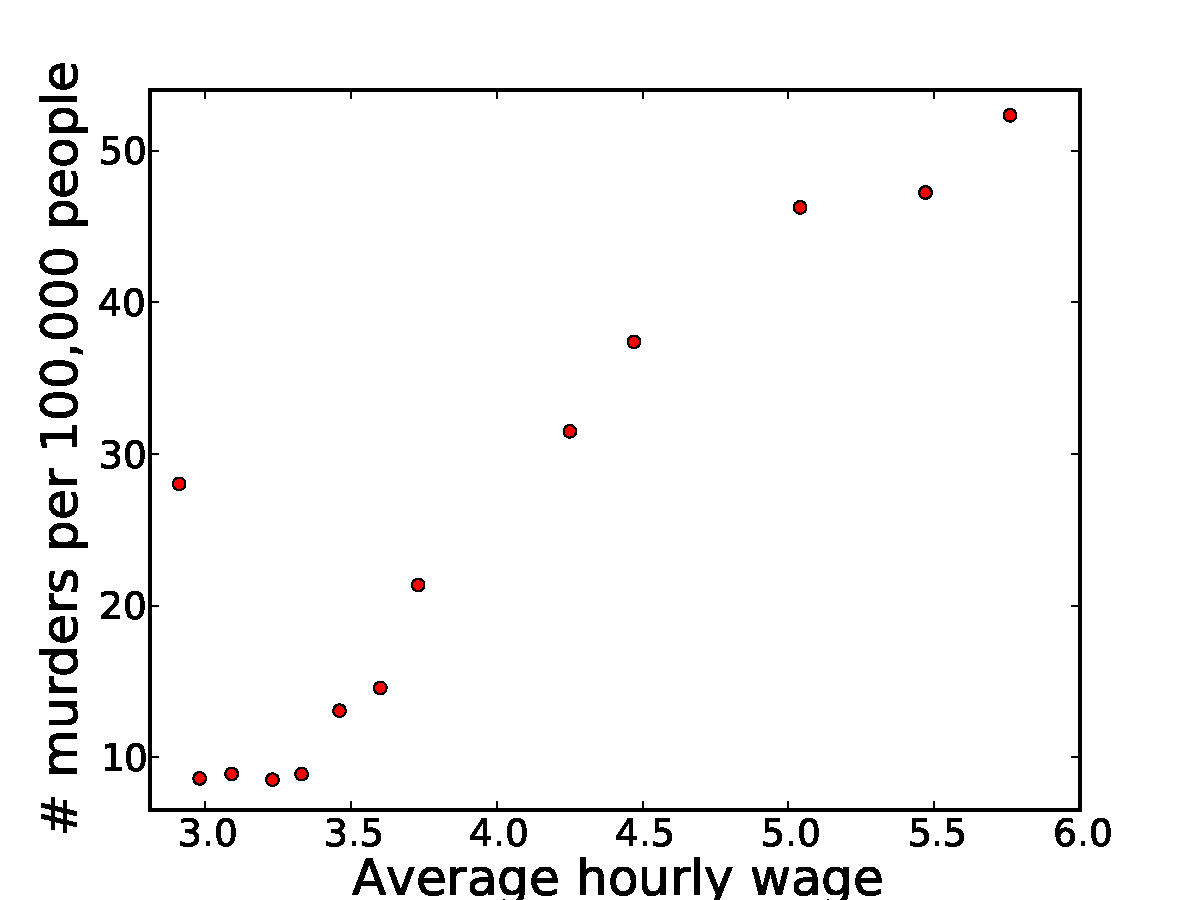
\includegraphics{figures/wage-murders.pdf}}
\scalebox{.4}{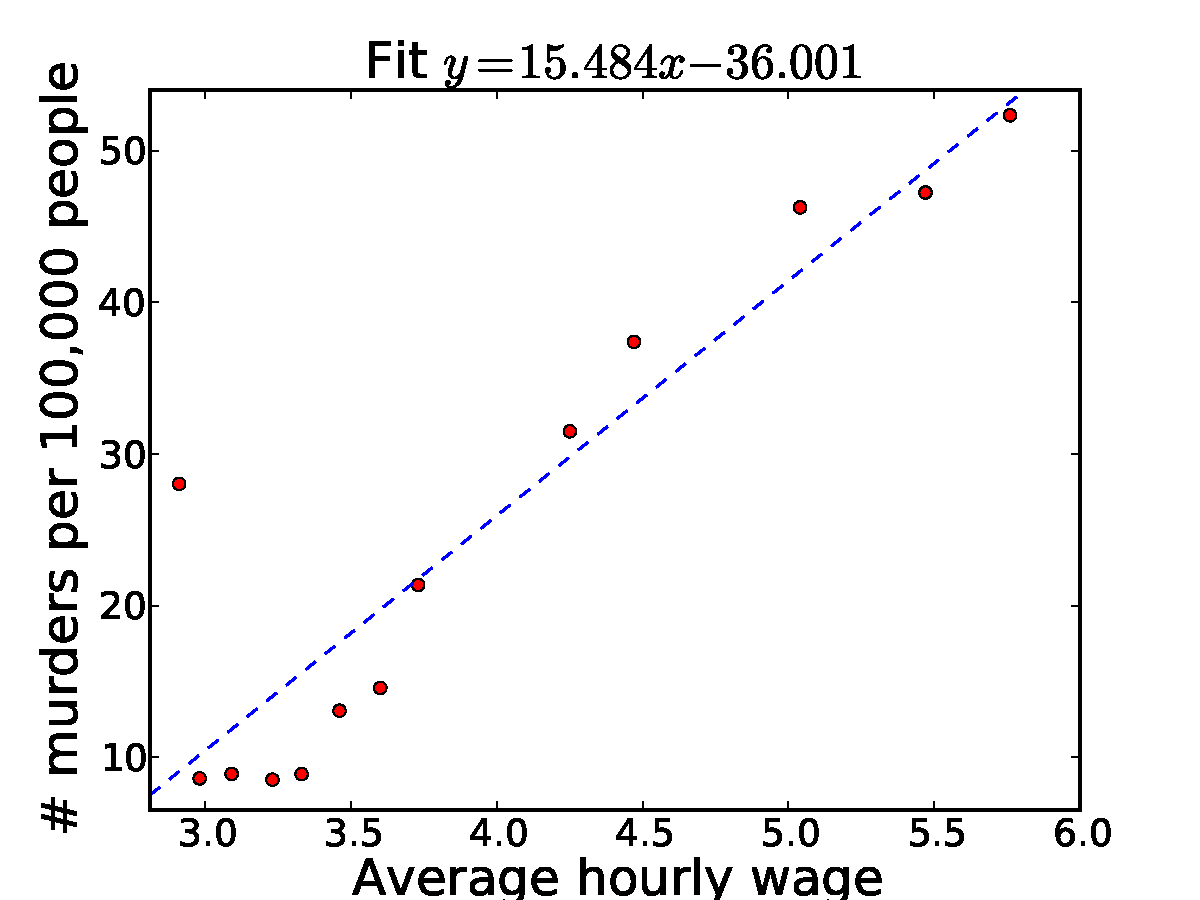
\includegraphics{figures/wage-murders-fit.pdf}}\\

\noindent Here, for example, $x_0 = 2.98$ and $y_0 = 8.6$.

{\em This might be a good point to remind everyone that correlation does not equal causation.}  I hardly think that paying people more makes them murderous, although I could see the opposite. ;)  Correlation is a {\em necessary} but not {\em sufficient} condition for causation. When you find a correlation, that gives you a candidate to check for cause-and-effect.

\subsection{Best fit line that minimizes squared error}

Recall the formula for a line from high school: $y = m x + b$.  We normally rewrite that using elements of vector $\vec{B}$ in preparation for describing it with vector notation from linear algebra. For simplicity,  though, we'll stick with scalar coefficients for now:

\[
y = b_1 + b_2 x
\]

The ``best line'' is one that minimizes some cost function that compares the known $y$ values at $x$ to the predicted $y$ of the linear model that we conjure up using parameters $b_1$, $b_2$. A good measure is the {\em sum of squared errors}. The cost function adds up all of these squared errors to tell us how good of a fit our linear model is:

\[
Cost(B) = \sum_{i=1}^{n}(\underbrace{b_1 + b_2 x_i}_\text{linear model} - \overbrace{y_i}^\text{true value})^2
\]

\noindent As we change the linear model parameters, the value of the cost function will change.  The following graphs shows the errors/residuals that are squared and summed to get the overall cost for two different ``curve fits.''

\scalebox{.35}{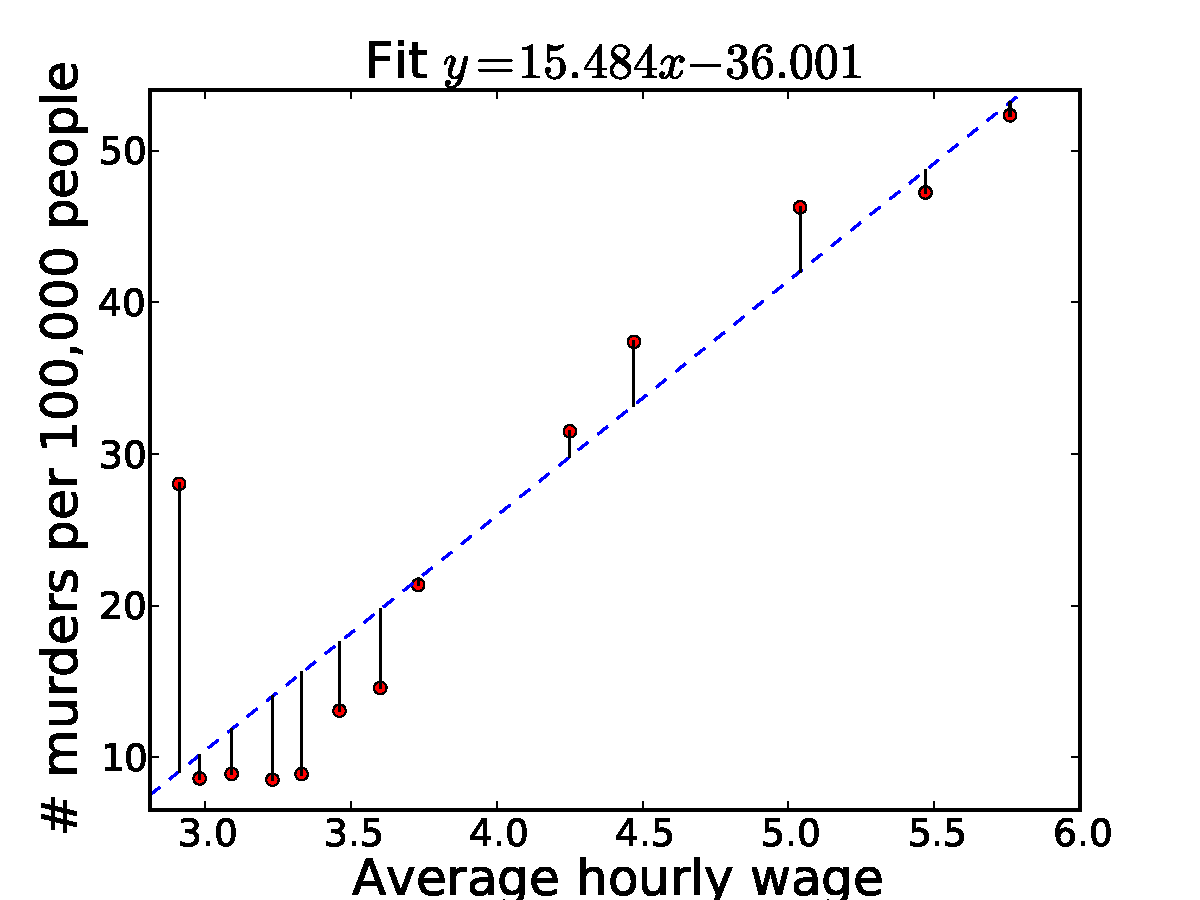
\includegraphics{figures/wage-murders-residuals.pdf}}
\scalebox{.35}{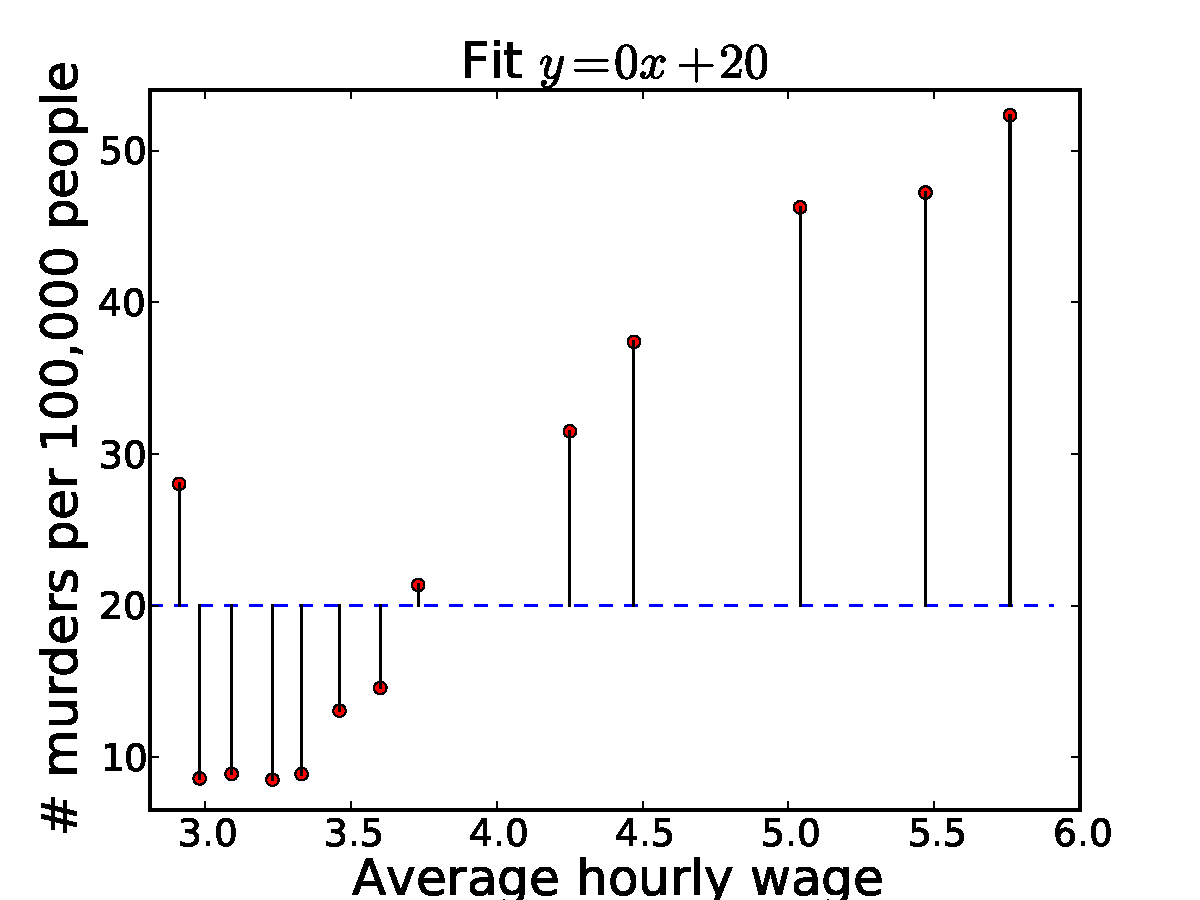
\includegraphics{figures/wage-murders-residuals-poor.pdf}}\\

\noindent The costs are 533.82 for the left and 3563.50 for the right.

The good news is that we know the cost function is a quadratic, which is convex and has an exact solution. All we have to do is figure out where the partial derivatives of the cost function are both zero; i.e., where the cost function flattens out (at the bottom).

\[\tag{Analytic solution to optimization}
\nabla Cost(B) = 0
\]

\noindent For our purposes, though, we'll reuse gradient descent to minimize the cost function.

To show our prediction model in action, we can ask how many murders  there would be in Detroit if the average salary were \$4.7? (Obviously, these wages are from 30 years ago.) To make a prediction, all we have to do is plug $x=4.7$ into $y = -36.001 + 14.484 x$, which gives us 32.074 murders.

\subsection{Gradient descent in 3D}

\cut{
{\em Make sure that you are using the latest Python, such as 2.7.8. I noticed that 2.7.5 does not draw heat maps and other things correctly.}
}

Before trying to minimize the cost function, it's helpful to study what the surface looks like in three dimensions, as shown in the following two graphs. The x and y dimensions or the coefficients of our linear model and the z I mentioned is the cost function.

\noindent \scalebox{.55}{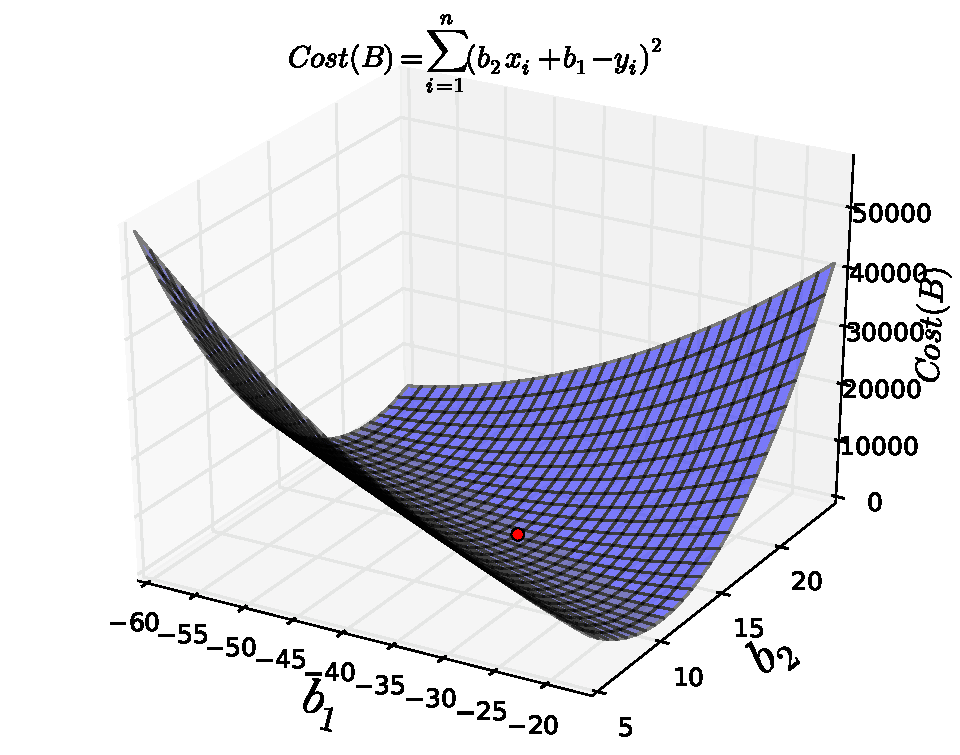
\includegraphics{figures/wage-murders-cost-3d.pdf}}
\scalebox{.45}{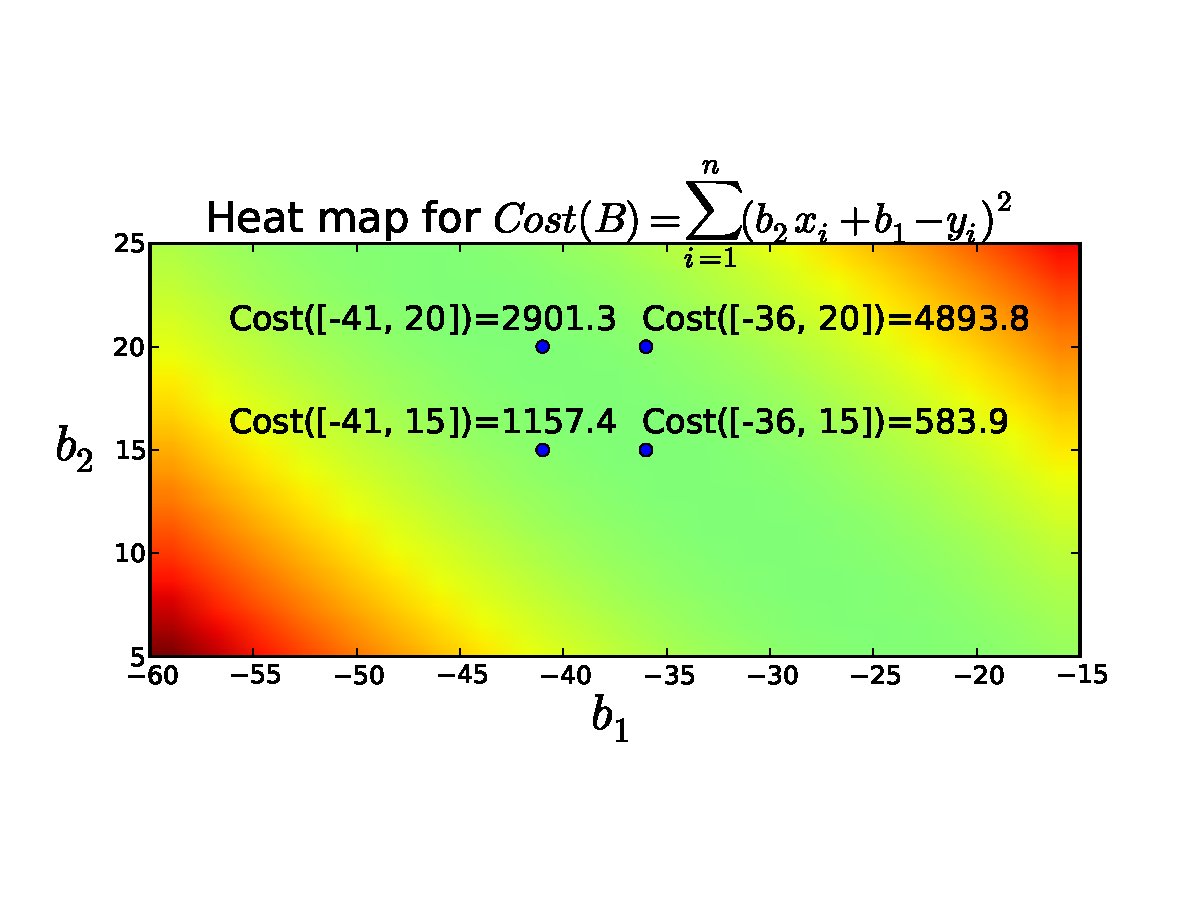
\includegraphics{figures/wage-murders-heatmap.pdf}}

What surprised me is that changes to the slope of the linear model's coefficient $b_2$, away from the optimal $b_2=15.484$, cost much more than tweaks to the y intercept, $b_1$. Regardless, the surface is convex and a unique solution exists. 

Unfortunately, based upon the deep trough that grows slowly along the diagonal of $(b_1,b_2)$, gradient descent takes a while to converge on the minimum. We will examine the path of gradient descent for a few initial starting point. Wikipedia says that the Rosenbrock function is a pathological case for traditional gradient descent and it looks pretty similar to our surface with its shallow valley:

\scalebox{.4}{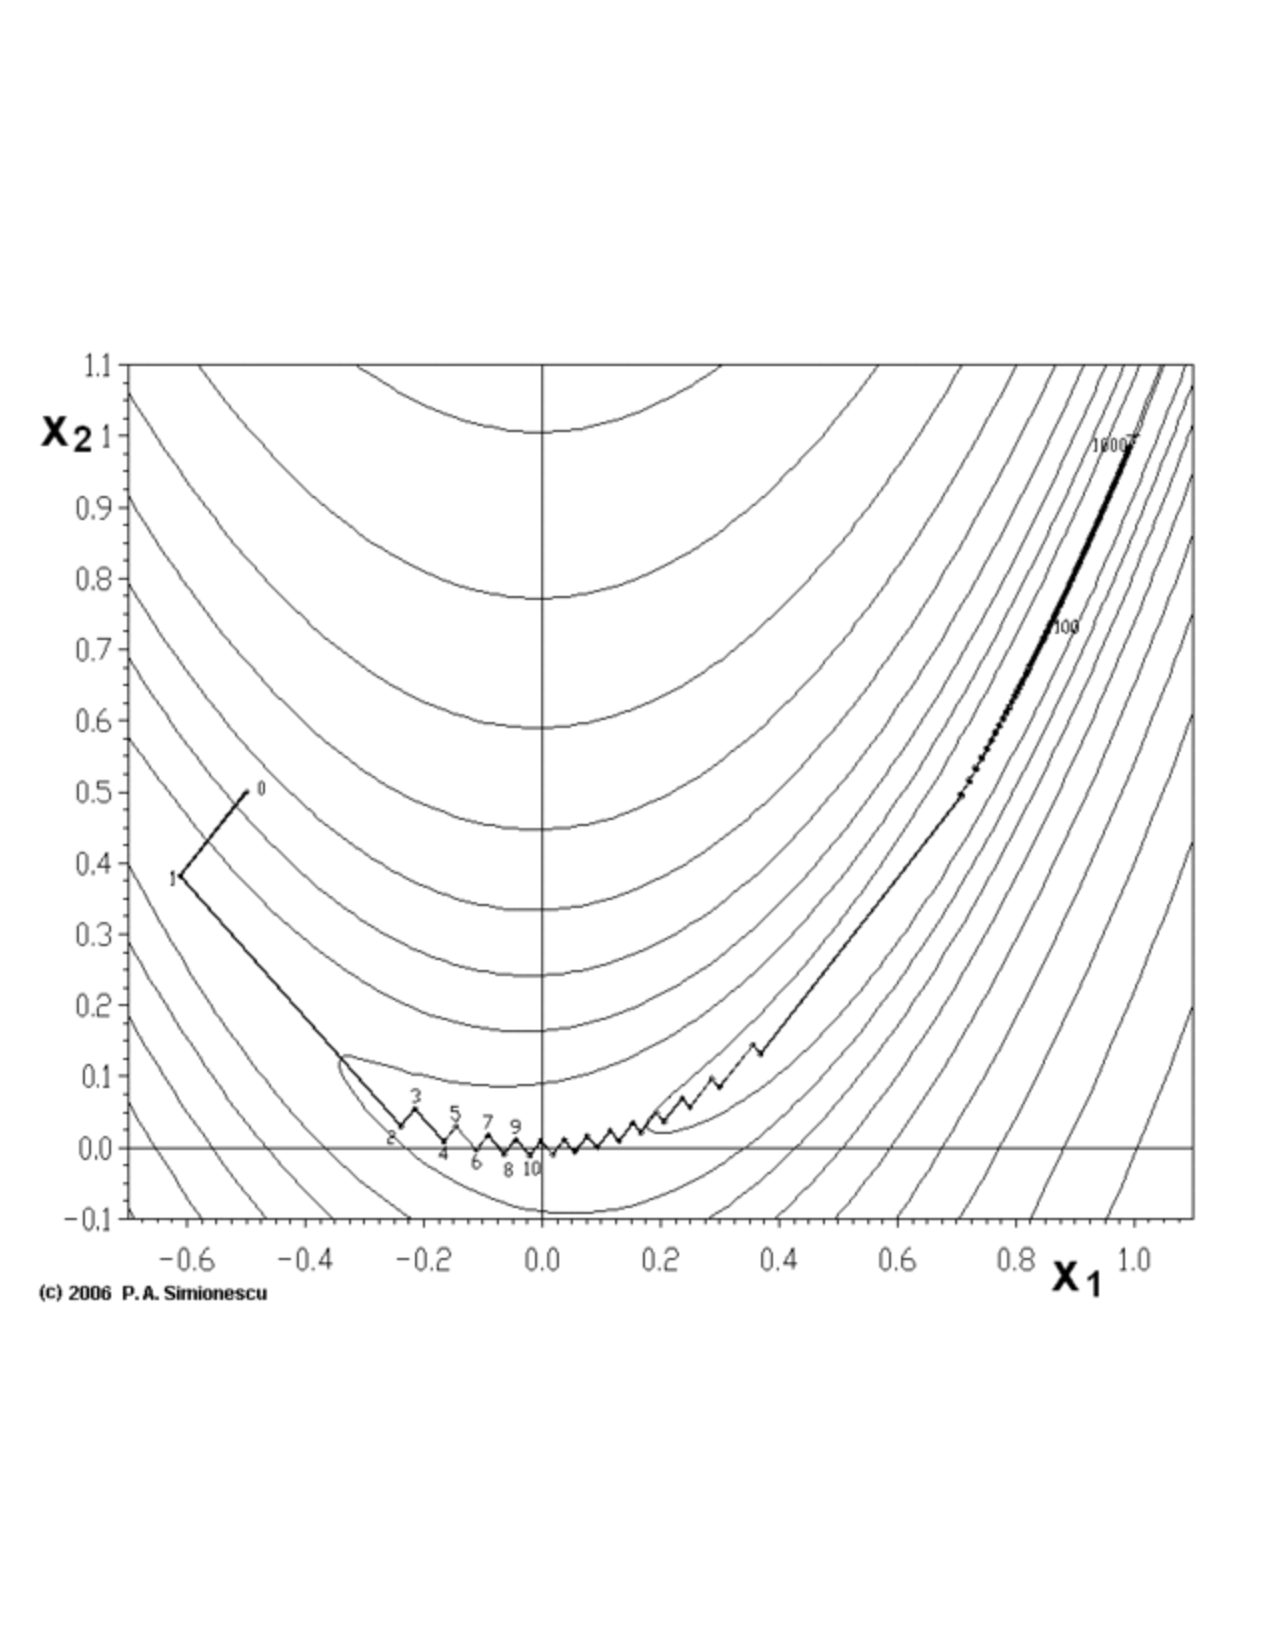
\includegraphics{figures/Banana-SteepDesc}}

The recurrence relation for updating our estimate of $\vec{B}=[b_1, b_2]$ that minimizes $Cost(\vec{B})$ is the same as our previous lab but with a vector instead of a scalar:

\[
\vec{B}_{i+1} = \vec{B}_i - \eta \nabla Cost(\vec{B}_i)
\]

\noindent where we will approximate vectors of partial derivatives with partial finite differences defined generically as:

\[
\nabla F(\vec{X}) =
\begin{bmatrix}
\frac{\delta}{x_1}{F(\vec{X})}\\
\frac{\delta}{x_2}{F(\vec{X})} \\
\end{bmatrix}
\approx
\begin{bmatrix}
\frac{F(\left[ x_1+h \above 0pt{x_2} \right]) - F(\vec{X})}{h} \\
\frac{F(\left[ x_1 \above 0pt{x_2+h} \right]) - F(\vec{X})}{h} \\
\end{bmatrix}
\]

\noindent In our case, we will compute the components of a finite difference vector $C'$ ignoring the division by the step $h$.

The minimization algorithm looks like:

\begin{enumerate}
\item Pick an initial $B_0$
\item let $B = B_0$
\item $C' = \left[ Cost(\left[ b_1+h \above 0pt{b_2} \right]) - Cost(B_i) \above 0pt Cost(\left[ b_1 \above 0pt{b_2+h} \right]) - Cost(B_i) \right]$
\item Let $B_{i+1} = B_i - \eta C'$
\item goto step 3 until $abs(Cost(B_{i+1})-Cost(B_i)) < precision$ or ``close enough'' by some measure
\end{enumerate}

Using a low learning rate, my solution takes 4843 steps starting from coordinate (-45,10) using a very small step size, which gives me a fairly decent approximation of the minimum: [-36.00066933  15.48414587] compared to the analytic solution [ -36.000625 15.484375 ]. Starting from about the same distance away in the shallow valley at (-45,25), my solution takes 5142 steps. Cutting my step size by 5x, takes 30463 steps but gives a slightly more precise result [-36.00063497  15.48432944]. Starting at (-45,25) takes 31958 steps. Surprisingly, when I start very close to the minimum at (-36,15), my solution takes 47350 steps and does not exactly give a more accurate result. ``{\em Your mileage may vary.}''

\noindent \scalebox{.45}{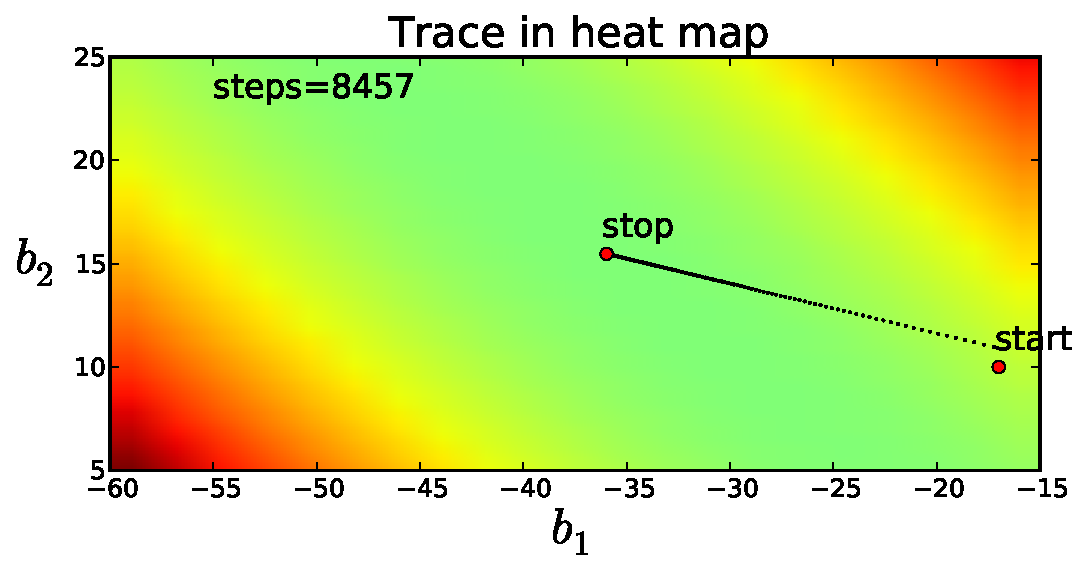
\includegraphics{figures/wage-murders-heatmap-trace1.pdf}}
\scalebox{.45}{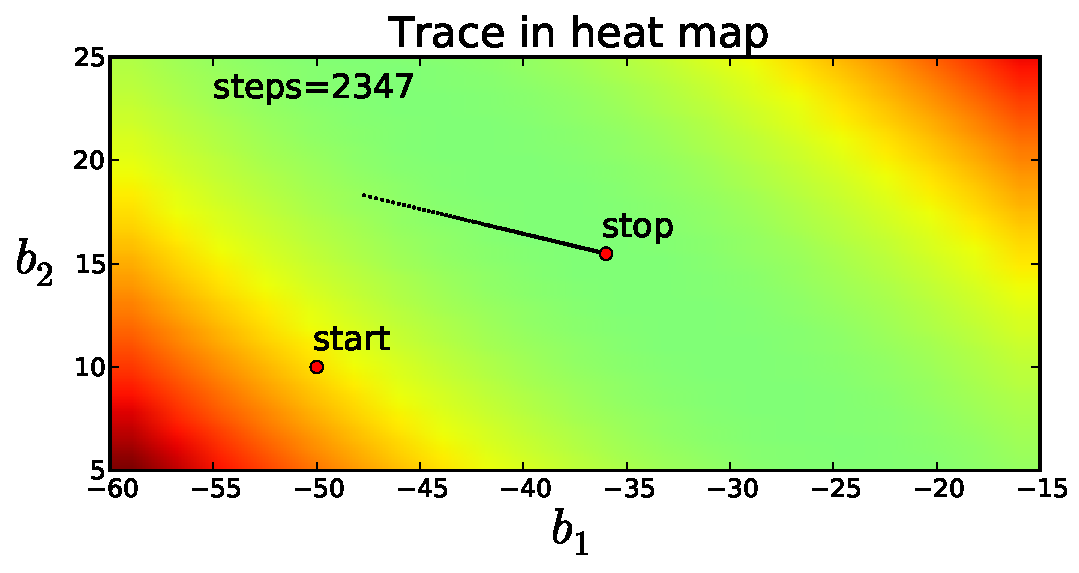
\includegraphics{figures/wage-murders-heatmap-trace2.pdf}}

\noindent \scalebox{.45}{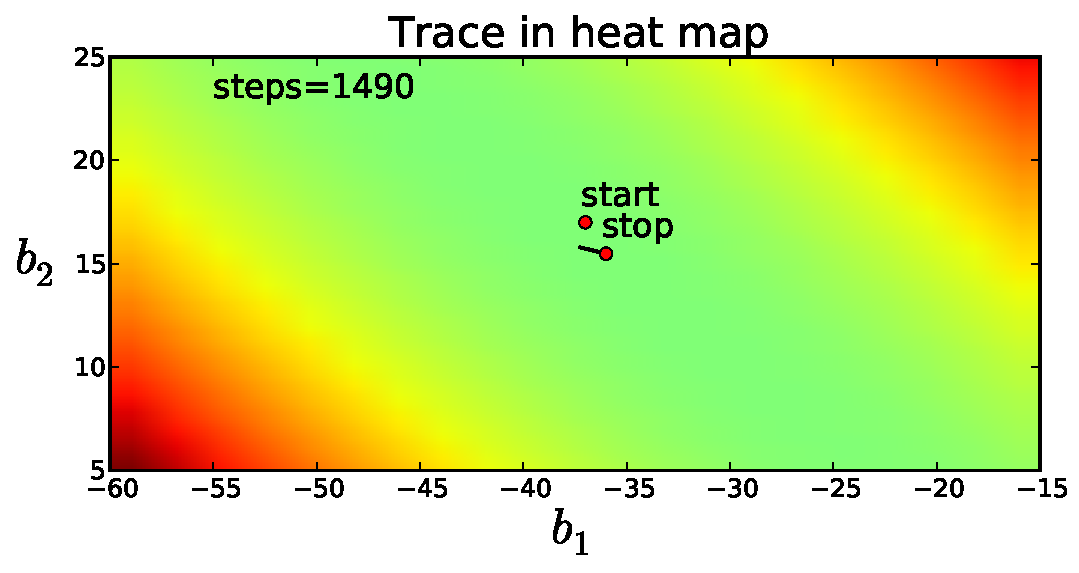
\includegraphics{figures/wage-murders-heatmap-trace3.pdf}}

When I crank up the learning rate and use a very small step size, my solution converges must faster and with the same accuracy. For example, with 10 times the learning rate as before, (-45,25) converges in 3193 steps instead of 31958 steps.

\section{Your task}

You will use gradient descent to solve the linear regression problem above, using the same data. As part of your final submission, you must provide heat maps with traces that indicate the steps taken by your gradient descent as I have shown above.  Have your program choose two random starting $B_0$ vectors to produce your heat maps, as always using your awesome and amazing {\tt runif\_()}.   Define a function called {\tt minimize} that takes the indicated parameters and returns the minimum $B$ parameters of your linear model, the number of steps, and the trace array of intermediate $B_i$ values.

\begin{pyverbatim}
def minimize(f, B0, eta, h, precision):
    trace = []
    B = B0
    steps = 0 
    while True:
        steps += 1
        if steps % 10 == 0: # only capture every 10th value
            trace.append(B)
        ...     
    ... 
    return (B, steps, trace)
\end{pyverbatim}

As an example, I call that function like this:

\begin{pyverbatim}
def f(B): # a helper function that simply adds in the default arguments of the data
    return Cost(B, HOURLY_WAGE, MURDERS)
# or, if you are one of the cool kids:
f = lambda B : Cost(B, HOURLY_WAGE, MURDERS)
(m,steps,trace) = minimize(f, B0, LEARNING_RATE, h, PRECISION)
heatmap(HOURLY_WAGE, MURDERS, trace=trace)
\end{pyverbatim}

Use {\tt pylab.imshow()} to draw the heat map whose $b_1$ are the $y$ intercepts, $b_2$ coordinates are the murders, and heat value is the cost of $x,y$.  It took me a while to figure out all of the crazy methods to draw the heat maps.  Plan on some frustration here.  Please show the information as I have shown in the graphs to make it easier to compare results and for me to grade. Hide all of your heat map construction and function like this:

\begin{pyverbatim}
def heatmap(X, Y, trace): # trace is a list of [b1, b2] pairs
    ...
\end{pyverbatim}

\noindent I plot the trace using:

\begin{pyverbatim}
plot(p[0], p[1], "ko", markersize=1)
\end{pyverbatim}

You will have to pick an appropriate step value $h$ to get a decent approximation of the derivative through finite differences that is large enough to avoid faulty results from lack of precision (subtracting two floating-point numbers in the computer results in a number with much less precision than the original numbers). You want that number to be small enough that your algorithm does not oscillate around the minimum. If the number is too big it will compute a finite difference that leads to $B_{i+1}$ leaping across the minimum to the other wall of the function. You must pick a learning rate $\eta$ that allows you to go as fast as you can but not so fast that it overruns the minimum back and forth. When I crank up my learning rate too far, I also see the algorithm go off into the weeds and stops with a minimum of [ -4.86000929e+10  -2.85744570e+12].

\section{Resources}

There is a lot of material out there on the web that can be helpful.

\begin{itemize}
\item \href{http://en.wikipedia.org/wiki/Finite_difference}{Finite difference at Wikipedia}
\item \href{http://research.microsoft.com/pubs/192769/tricks-2012.pdf}{Stochastic Gradient Descent Tricks}
\item \href{http://apps.nrbook.com/fortran/index.html}{Numerical recipes (See Chap 10 on minimization of functions)}
\item \href{http://adl.stanford.edu/aa222/Lecture_Notes_files/AA222-Lecture2.pdf}{Single verbal minimization in line searches}
\item \href{http://cs229.stanford.edu/notes/cs229-notes1.pdf}{Andrew Ng's CS229 Lecture notes}
\item \href{http://people.duke.edu/~ccc14/pcfb/analysis.html}{Data analysis with Python}
\end{itemize}

\section{Deliverables}

{\bf You must tweak the step size and other parameters so that your results agree with the first four decimal points of the analytic solution [-36.000625000000007, 15.484375].}

Please submit the following via canvas:
 
\begin{itemize}
\item A PDF of your graph with two visible traces on two heat maps or the same heat map if the traces are clear. The graph should include the start, stop location and the number of steps as I have done on mine. As part of your PDF, please indicate the $B$ parameters you compute with your minimize function.
\item Please put all of your "main" program inside of the usual: {\tt if \_\_name\_\_ == '\_\_main\_\_':}.
\item Your {\tt regression\_descent.py} code and {\tt varunif.py}.
\end{itemize}

\end{fullwidth}

